\chapter{Morse Code Reader} \label{chap:morsecodereader}
\section{Case Description}
This model represents a device for decoding a message presented in
Morse code.  Morse code is a system which uses one or more ``dots''
and ``dashes'' to represent standard Latin characters.  The dots and
dashes can be represented as long or short flashes of light, as long
and short audible tones, or as long and short marks on paper.  In this
case the message to be decoded is delivered as long and short marks on
a strip of light-coloured tape.  The marks represent dots if they are
narrow and dashes if they are wide.  The decoder has a sensor able to
detect light and dark on the tape and a motor which is capable of
moving the tape so that it passes in front of the sensor.  When it is
ready to read a message, the decoder produces a signal to the motor to
move the tape continuously past the sensor, and periodically collects
a reading from the sensor which indicates whether a light or a dark
colour is currently visible on the tape.  These readings are collected
and used to determined whether the tape is currently displaying a dot,
a dash or a space.  Information on dots and dashes and the spaces
between them is collected in turn, and then translated into standard
Latin characters using a lookup table.  Figure \ref{fig:morsereader}
presents a diagram of the Morse decoder device, showing the tape with
the message, the motor that moves the tape, the sensor to read the
tape and the controller which is linked to both sensor and motor.

\begin{figure}[!ht]
\centering
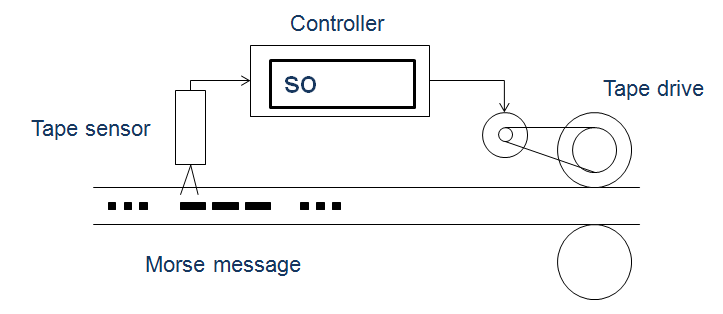
\includegraphics[width=8cm]{morseCodeReader/MorseTapeReader.png}
\caption{Overview of the Morse decoder \label{fig:morsereader}}
\end{figure} 

It's assumed that the message which is encoded is preceded by a
standard Morse ``attention'' sequence and is followed after its
completion by a standard ``end of work'' sequence.  The following
assumptions are also made:
\begin{itemize}
\item a dash is three times the length of a dot
\item there is a space (no signal) the same length as a dot between
  dots and/or dashes
\item there is a space the length of three dots between two separate
  ASCII characters
\item that there is space the length of seven dots between two ASCII
  words
\end{itemize}
The exact length of the mark used to represent a dot and the mark used
to represent a dash are unknown and must be calculated by the decoder
before message can be decrypted.  Therefore the Morse code reader
firstly detects the ``attention'' sequence that precedes the message,
and from this it performs some calibration to determine the width of a
dot and the width of a dash. The width is determined in terms of the
number of samples taken which were not background colour.

\section{Contract} The contract for the Morse decoder model contains two variables of type
\keyw{real}. A \emph{monitored} variable, \texttt{morseSensorShared},
represents input from the sensor that detects light and dark.  A
\emph{controlled} variable, \texttt{motorVoltageShared}, is used to
produce a signal to the motor which moves the tape past the sensor.

The contract also includes two shared design parameters of type
\keyw{real}: \texttt{AToDResolutionBits} and \texttt{AToDNoiseBits}.
These are used for configuring the noise and resolution of the input
data so that fault tolerance mechanisms may be exercised.

\section{Discrete-event} The DE model contains an
\texttt{AbstractMorseReader} class, which assumes the role of a
controller and has the main thread of control.  At runtime a concrete
implementation of the \texttt{Abstract\-MorseReader} is provided by the
\texttt{ModalController}, which in turn instantiates abstract classes
to represent the actuator for the motor
(\texttt{AbstractActuatorReal}) and the sensor
(\texttt{AbstractFilteredSensorReal}). At run-time concrete
implementations of these classes are provided by the
\texttt{ActuatorReal} class and the \texttt{FilteredSensorReal} class
respectively. Designing a controller that primarily handles abstract
classes makes it easier to replace or alter the concrete
implementation at a later date if necessary.

\texttt{ActuatorReal} allows the DE model to set the voltage for the
motor to move tape past the sensor.  \texttt{FilteredSensorReal}
allows the sample size to be set (how many samples are used to
determine if something is black or white, determined during
calibration), as well as reading in a value from the sensor.

Some other classes are also provided.  The \texttt{MorseLookup} class
provides a method to translate a sequence of dots and dashes into
ASCII characters.  The \texttt{DotDashOrSpace} provides methods to
check for the existence of a dot, a dash or a space given some input
from the sensor.

The process of decoding the Morse message involves a number of
different stages, or modes, of operation.  The
\texttt{ModalController} class stores a variable,
\texttt{controllerMode}, which is of type
\texttt{AbstractControllerMode} and is responsible for providing the
methods to be employed during the current mode.  During initial
operation \texttt{ControllerModeMeasureSignalNoise} provides the
concrete implementation of \texttt{AbstractControllerMode}; this class
examines the input whilst the tape remains stationary, in order to
determine the signal to noise ratio.  A higher level of noise results
in a lower overall speed being selected for reading the rest of the
tape.  The motor is off during this calibration phase but on for all
other phases.  Next the concrete implementation of
\texttt{AbstractControllerMode} is replaced with the
\texttt{ControllerModeMeasureDotDash\-Length} class, which provides
methods to handle the calibration process of identifying the attention
sequence and measuring dot length.  Then the mode changes again and
the functionality of the \texttt{AbstractControllerMode} is provided
by the concrete implementation \texttt{ControllerMode\-ReadMessage}.
This mode class provides methods to collect sensor readings at
appropriate sampling intervals and to translate collections of dots
and dashes.  Finally the concrete implementation is provided by
\texttt{ControllerModeIdle}, which simply ensures that the motor
voltage is set to zero.

The \texttt{AbstractMorseReader} (the controller class) is deployed
onto a single CPU by the \texttt{System} class.

\section{Continuous-time} 
The CT model consists of three main blocks, \texttt{controller},
\texttt{Motor} and \texttt{morseSensor}, in addition to a single block
which represents the plant. The \texttt{Controller} block handles the
interface between the CT model and the DE model. The \texttt{Motor}
block resides between the \texttt{Controller} and the plant, and
accepts an input which is the voltage to be applied to the motor
itself.

The \texttt{morseSensor} block represents the sensor and accepts some
input from the plant, handles A/D conversion and produces an output
for the \texttt{Controller}.  The output indicates how dark was the
currently visible section of tape.

\section{Usage} 
The model uses some data files to represent tapes with Morse code
messages, and some examples are provided with the model.  Each message
is represented in three files: an image is provided purely for the
user to visualise what the sensor should be able to see; a file
\emph{message.txt} represents the same data, but is actually used by
the sensor to generate data; and a further file
\emph{message-length.txt} is used to ensure that the image is
displayed to scale.  One way to get started with the model is to try
decoding different messages.  This simply involves running the model
with the included sample messages.  A further step could be to
generate your own message files and test out the decoding process. A
Java \emph{.jar} file, \texttt{TextToMorseTape.jar}, is included
alongside a readme file alongside the CT model.  This jar file can be
used to generate the three message files required, given some text.

The model needs to deal with the difficulty of reading a signal which
is delivered against some background noise.  The model copes with this
by analysing the signal-to-noise ratio before it begins and setting a
lower speed for reading more ``noisy'' data.  This allows the decoder
to take more samples for each of the dot or dash characters,
increasing confidence that data is accurately interpreted.  An
interesting experiment for the Morse decoder model involves varying
the amount of background noise that it is expected to cope with.  This
is set as a shared design parameter in the contract, and can be set at
runtime by opening the Debug configuration for the \DESTECS model.
Running the model with the same input files and higher levels of
background noise should see a slower decryption process because the
tape moves more slowly and more samples are collected, whilst
decreasing the background noise should see the decoder produce the
decrypted message more quickly.
